\documentclass{article}

\usepackage{fancyhdr}
\usepackage{extramarks}
\usepackage{amsmath}
\usepackage{amsthm}
\usepackage{amsfonts}
\usepackage{tikz}
\usepackage[plain]{algorithm}
\usepackage{algpseudocode}

\usetikzlibrary{automata,positioning}

%
% Basic Document Settings
%

\topmargin=-0.45in
\evensidemargin=0in
\oddsidemargin=0in
\textwidth=6.5in
\textheight=9.0in
\headsep=0.25in

\linespread{1.1}

\pagestyle{fancy}
\rhead{\firstxmark}
\lfoot{\lastxmark}
\cfoot{\thepage}

\renewcommand\headrulewidth{0.4pt}
\renewcommand\footrulewidth{0.4pt}

\setlength\parindent{0pt}

%
% Create Problem Sections
%

\newcommand{\enterProblemHeader}[1]{
    \nobreak\extramarks{}{Problem \arabic{#1} continued on next page\ldots}\nobreak{}
    \nobreak\extramarks{Problem \arabic{#1} (continued)}{Problem \arabic{#1} continued on next page\ldots}\nobreak{}
}

\newcommand{\exitProblemHeader}[1]{
    \nobreak\extramarks{Problem \arabic{#1} (continued)}{Problem \arabic{#1} continued on next page\ldots}\nobreak{}
    \stepcounter{#1}
    \nobreak\extramarks{Problem \arabic{#1}}{}\nobreak{}
}

\setcounter{secnumdepth}{0}
\newcounter{partCounter}
\newcounter{homeworkProblemCounter}
\setcounter{homeworkProblemCounter}{0}
\nobreak\extramarks{Problem \arabic{homeworkProblemCounter}}{}\nobreak{}

%
% Homework Problem Environment
%
% This environment takes an optional argument. When given, it will adjust the
% problem counter. This is useful for when the problems given for your
% assignment aren't sequential. See the last 3 problems of this template for an
% example.
%
\newenvironment{homeworkProblem}[1][-1]{
    \ifnum#1>0
        \setcounter{homeworkProblemCounter}{#1}
    \fi
    \section{Problem \arabic{homeworkProblemCounter}}
    \setcounter{partCounter}{1}
    \enterProblemHeader{homeworkProblemCounter}
}{
    \exitProblemHeader{homeworkProblemCounter}
}



%
% Homework Details
%   - Title
%   - Due date
%   - Class
%   - Section/Time
%   - Instructor
%   - Author
%

\newcommand{\hmwkTitle}{Homework\ \#1}
\newcommand{\hmwkName}{Fast Trajectory Replanning}
\newcommand{\hmwkDate}{February 17, 2023}
\newcommand{\hmwkClass}{CS 440: Introduction to Artificial Intelligence}
\newcommand{\hmwkClassInstructor}{Professor Abdelsam Boularias}


%
% Title Page
%

\title{
    \vspace{2in}
    \textmd{\textbf{\hmwkClass}}\\
    \textmd{\hmwkTitle\ \hmwkName}\\
    \vspace{0.1in}\small{\hmwkDate}\\
    \vspace{0.1in}\large{\textit{\hmwkClassInstructor}}
    \vspace{3in}
}

\author{
    \textbf{Jay Patwardhan} {208001851}\\ 
    \textbf{Alan Wu} {208000574}\\ 
    \textbf{Neel Shejwalkar} {RUID}
}
\date{}

\renewcommand{\part}[1]{\textbf{\large Part \Alph{partCounter}}\stepcounter{partCounter}\\}

%
% Various Helper Commands
%

% Useful for algorithms
\newcommand{\alg}[1]{\textsc{\bfseries \footnotesize #1}}

% For derivatives
\newcommand{\deriv}[1]{\frac{\mathrm{d}}{\mathrm{d}x} (#1)}

% For partial derivatives
\newcommand{\pderiv}[2]{\frac{\partial}{\partial #1} (#2)}

% Integral dx
\newcommand{\dx}{\mathrm{d}x}

% Alias for the Solution section header
\newcommand{\bruh}{\textbf{\large Solution}}
\newtheorem*{solution*}{Solution}
\newenvironment{solution}{\begin{solution*}}{{\finishline} \end{solution*}}


% Probability commands: Expectation, Variance, Covariance, Bias
\newcommand{\E}{\mathrm{E}}
\newcommand{\Var}{\mathrm{Var}}
\newcommand{\Cov}{\mathrm{Cov}}
\newcommand{\Bias}{\mathrm{Bias}}

\begin{document}

\maketitle

\pagebreak

%Part 0%
\begin{homeworkProblem}
    \textbf{\large Setting Up Our Environments}\\\\
    Language used: Python
    
    The maze is visually depicted just like the sample shown by Prof Boularias, with spaces depicting open cells, X depicting blocked cells, A representing the current location, T representing the target, and dots representing the path taken.
    
    The graph structure was generated as such: a cell containing its coordinate, display, and other important values for executing the searches. These cells were stored in order inside an array, for O(n) printing time with respect to the number of cells. Blockings were randomly generated through DFS starting at a random node with a 30 percent probability of being blocked.
    
    We have also constructing our own minheap/priority queue class utilizing our graph structure to store cells in the array, and comparing by accessing the f and g values of the cells with respect to tie breaking.
\end{homeworkProblem}

\pagebreak

%Part 1%
\begin{homeworkProblem}
    \textbf{\large Understanding the Methods}\\\\
    \part 

    Explain in your report why the first move of the agent for the example search problem is to the east rather than to the north given that the agent does not know initially which cells are blocked.

    \begin{solution*}
    This is because in our search problem, the agent knows information about the blockage status of its direct neighbors, so the cell above, below, left, and right of it. Furthermore, for each new step it takes placing it in a new spot, it again obtains the status of each of its neighbors, so it will continuously update its knowledge of which cells are blocked as it moves along. Thus, in the example search problem, the agent at its starting point recognizes that its neighbors to the right and above are blocked, and its neighbor below is out of bounds and thus doesn't exist, and thus it can only move to the east as its first move.
    
    In our graph implementation, the cost associated with moving to a known blocked cell increases to infinity. Furthermore, we closely follow the pseudocode given in the writeup, with some modification. Thus, $g(s_{goal}) = \infty$, and when adding the right and above cells to the OPEN list, their f values are stored as g(s) + c(s,a), but $c(s,a) = \infty$ because these cells are blocked, thus their f values are $\infty$. It then follows that the condition of the while loop isn't satisfied for these two cells in ComputePath(), as $g(s_{goal}) == min(OPEN) = \infty$ for these two cells, and thus ComputePath() terminates, and never considers a path from the right or above. Thus, it follows that the first move of the agent for the example search problem is to the east, as it contains an f value that is not $\infty$ and thus continues the loop.
    \end{solution*}

    \part

    This project argues that the agent is guaranteed to reach the target if it is not separated from it by blocked cells. Give a
convincing argument that the agent in finite gridworlds indeed either reaches the target or discovers that this is impossible
in finite time. Prove that the number of moves of the agent until it reaches the target or discovers that this is impossible is
bounded from above by the number of unblocked cells square

    \begin{solution*}
    We note that every A* search either finds a path or returns that this is not possible in finite time by design. The implementation of a closed list also prevents infinite loops between the same cells in search of a path that may or may not exist. Thus, if a path exists for the agent in view  of the blockages that are known to it, A* will find this in finite time. If the path found turns out to be blocked, A* will pivot and find another path in view of the blockages that are known to it now. Inductively, since the gridworld is finite and the number of blockages are thus finite, the agent will find a path, if it exists. Furthermore, there is no possibility of searching the same path/paths multiple times and not succeeding, since the blockages that are revealed through a failure will update the path, and the newly found path will not be the same as the previously determined best path because it won't go through a blockage. Thus, each new optimal path determined by A* in a successive run is unique, as it will either succeed (trivial case) or run into a block, and the next path found will not go through this block. Since the number of blocks are finite, this process will terminate when a path is found. If no path exists, then A* terminates by design. 


    It is important to determine whether this termination happens in finite time. Thankfully, it does. By the process above, all blocked cells will be found, or a solution will be found, whichever comes first, and both will occur in finite time. Once all blockages are found, and if there still doesn't exist a path, then A* by definition will terminate and return that no path exists. Thus, repeated A* will also terminate in finite time.
    \end{solution*}
    


   
\end{homeworkProblem}

\pagebreak

%Part 2%
\begin{homeworkProblem}
    \textbf{\large The Effects of Ties}\\\\
    For the example search problem, the start and end cell are at the largest possible Manhattan distance away, a distance of 8. It is also good to note that since there are no blockages, A* will succeed on the first run. Furthermore, each step contains a cost of 1, since there are no blocked cells. Thus, for every step that is moved closer to the target, g increases by 1, and h decreases by 1. Thus, for any path from start to finish, where no moves are made in a direction away from the target (the h value of the cell we move to is never greater than the g value of the current cell), the f value of each cell along the path is constant at 8.
    This is where tiebreaking comes in. If we favor large g values, we will consider first the path which a larger g value, meaning a path which has more nodes to it. Thus, this will expand less nodes, as A* will consider the nodes which are closer to the target first, and continue expanding this path in particular. This tiebreaking expands around 8-11 cells on average. However, when we favor small g values, we consider newer paths first which stem from the origin, and thus we expand slowly, like a BFS expanding out from the origin. Since our agent is at the farthest away possible location from the target, the agent will expand each cell, and A* expands 25 cells per run. The runtime is also slower when considering smaller g values due to this.
    \newline\newline
    Tiebreaking is done by gathering the indices of g values of all cells whose f value is equal to the f value at the top of the heap, and finding the indices of the maximum/minimum g value through its appropriate max/min Python function. If ties persist, we shuffle this array of indices all containing the max/min value, and choose at random an index, which we follow to its cell and denote this the cell to expand. In the priority queue, we swap this cell with the top, pop the top (which is now this cell), and reheapify. Since we swapped two cells with the same f value, we don't need to reheapify after the swap, only after the delete.
    \newline\newline
    We now turn to testing tie breaking by running repeated forward A* 50 times on a 101x101 grid and compare the runtime on each grid based on favoring big g values or smaller g values inside the Minheap. The stats for favoring big g are: mean: 0.3710785; median 0.133859; std 0.5682413.
    The stats for favoring small g are: mean: 0.865509; median 0.22789049; std 1.557079. As we can see, in general selecting larger g values is favored, although the difference is not quite large. However, there are quite noticeable outliers for the case where we favor small g values, and these are the cases in which we expand most cells on the board, similar to the example problem we explained above. Thus, while both runtimes are similar, we avoid cases where we expand each cell by favoring larger g values when tiebreaking. We show these outlier cases below, where the top grid is for larger g values, and the bottom grid is for smaller g values.
    \newline
    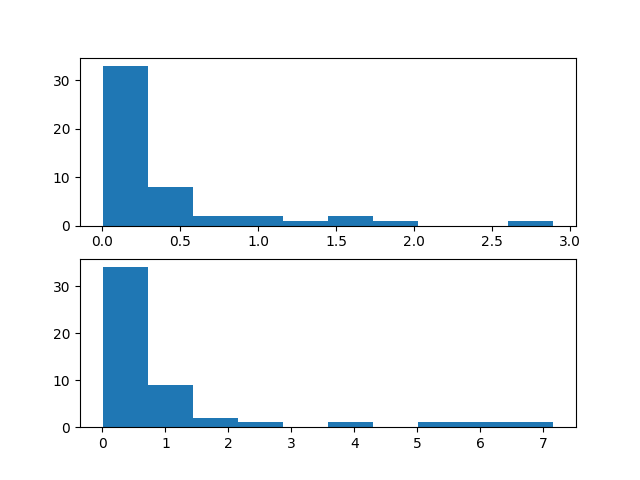
\includegraphics{big_g_vs_small_g.png}
    
   
\end{homeworkProblem}

\pagebreak

%Part 3%
\begin{homeworkProblem}
    \textbf{\large Forward vs. Backward}\\\\
    Summary: We find that repeated forward A* works as well as repeated backward A* IF THE GRID SIZE IS SUFFICIENTLY SMALL. For grid size 10x10, and up to even 50x50, we find that the median times and statistics for repeated forward and backward A* are very similar to each other. However, for large grid sizes like the 101x101, whose data is shown below, we find that there is a more significant difference in algorithmic runtime. In particular, the outliers for mazes for which a path doesn't exist takes a particularly larger amount of time for the backward case. To be entirely honest, we are not sure why such behavior happens for large nxn cases but not in small cases, since the algorithm is basically identical. A particularly good result is that of finding identical behavior with regards to runtime when the grid size is small.
    \newline \newline
    We use a 101x101 grid size, and perform a repeated forward A* search against an adaptive A* search on 25 different grids. The duplicate grid used to test adaptive A* was used using a Python deep copy, with some modification.
    The stats for forward are: mean: 0.238084736; median 0.11718643; std 0.3508612. 
    The stats for backward are: mean: 1.4704239; median 0.681670547; std 1.996149. In general, the median search time is faster than the mean search time, and is a more reliable indicator when comparing performances because means may get skewed.
    Furthermore, as seen below, we find that the histograms for the time taken to find a solution is slightly different, as although they have the same shape, repeated backward A* takes longer to execute. Repeated forward A* is on the top, repeated backward A* is on the bottom.
    \newline
    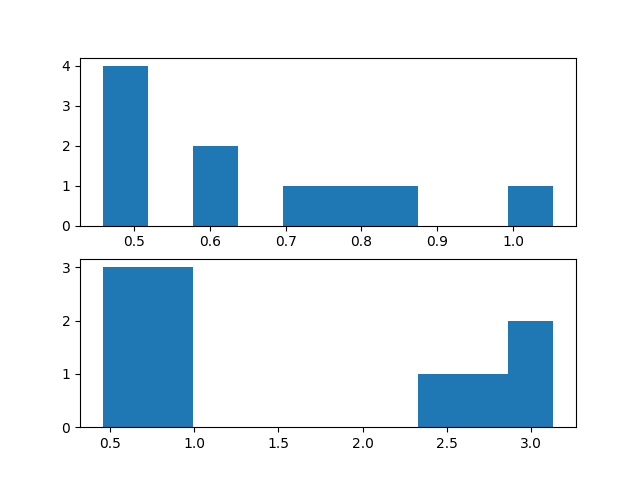
\includegraphics{forward_vs_backward.png}
\end{homeworkProblem}

\pagebreak

%Part 4
\begin{homeworkProblem}
    \textbf{\large Heuristics in the Adaptive $A ^{*}$}\\\\

    \part
    
        The project argues that “the Manhattan distances are consistent in
gridworlds in which the agent can move only in the four main compass directions.” Prove that this is indeed the case.
    \begin{solution*}
        We must show that for $s,s' \in S, h(s) \leq h(s') + c(s,s')$. If we run into a blocked cell, then $c(s,s') = \infty$, and this holds. If we run into an unblocked cell, then $c(s,s') = 1$, and this holds, since the difference in Manhattan distance between two adjacent cells is necessarily 1. Thus, regardless of whether the move from s to s' lands you closer to the target or not, since the distance is 1, this is recovered by the cost function. If the move is not optimal, then this holds trivially since c(s,a) is nonnegative.
    \end{solution*}

    \part
    
        Furthermore, it is argued that “The h-values $h_{new}(s)$ ... are not only admissible but also consistent.” Prove that Adaptive A*
leaves initially consistent h-values consistent even if action costs can increase.

    \begin{solution*}
        Note that this boils down to 4 cases: for $s,s' \in S$, either both s and s' have heuristic $h_{new}$, both have the old heuristic h, s has $h_{new}$ and s' doesn't, or vice versa. Note for all proofs that c(s,s') denotes the cost of moving from s to s', and s and s' are adjacent cells. The case for arbitrary s and s' follows by induction by considering the path from s to s' using intermediary t values.
        
        \begin{itemize}
            \item Case 1: s and s' have the old heuristic h. Then, since we assume the old heuristic h is consistent, our inequality holds trivially.
            \item Case 2: s and s' have the new heuristic $h_{new}$. $h_{new} = g(target) - g(s)$, and we note that g(s) has the triangle inequality: $g(t) \leq g(t') + c(t,t') for t,t' \in S$. This is because g discovers the shortest A* path from a state to the target. Thus, for any two adjacent cells t and t', $g(t) - g(t') \leq 1$. Suppose for contradiction that the distance was 2 or more, call $g(t) = a$ and $g(t') = a + k, k \geq 2$. Then, we may find a shorter path from t' to the target by moving from t' to t, which would make $g(t') = a + 1$, which contradicts our paths found by A* being optimal. Thus, $g(t) - g(t') \leq 1, and c(t,t') = 1$ since both cells are unblocked. Now, we note that $h_{new}(s) \leq h_{new}(s') + c(s,s')$ becomes $g(target) - g(s) \leq g(target) - g(s') + 1$, which becomes $g(s') \leq g(s) + 1$, which we have proven to hold since g has the triangle inequality for $c(s,s') = 1$.
            \item Case 3: s has the old heuristic while s' has the new heuristic. We have that $h(s) <= h_{new}(s) for s \in S$, thus we have that $h(s) \leq h(s') + c(s,s') \leq h_new{s'} + c(s,s')$.
            \item Case 4: s has the new heuristic while s' has the old heuristic. This means that s' wasn't expanded, meaning that its f value was less than any of the expanded f values including that of the target, and since the f value of the target when reached by the previous A* search is equal to g(target) since h(target) is 0, it holds that for all cells $s \in S$ not expanded by the A* search, $g(target) <= f(s)$. Thus, $g(target) <= f(s')$ in this case. We also note that the triangle inequality for g proved in Case 2 holds, and will be use here. Now, we have that $h_{new}(s) = g(target) - g(s) \leq f(s') - g(s) = g(s') + h(s') - g(s) \leq g(s') + h(s') - g(s') + c(s,s') = h(s') + c(s,s')$. Thus, $h_{new}(s) \leq h(s') + c(s,s')$.
        \end{itemize}

        Thus, for all cells, regardless of if they were affected by the heuristic change or not, the triangle inequality holds, and thus the new h values are consistent. Now, we denote all h values, whether they're updated h values or not, to be h. h is consistent. Suppose we increase the cost, so $c(s,s') \leq c'(s,s')$. Then, it follows that $h(s) \leq h(s') + c(s,s') \leq h(s') + c'(s,s')$. Thus, these h values are consistent even under increasing costs.
    \end{solution*}
    
\end{homeworkProblem}

\pagebreak

%Part 5
\begin{homeworkProblem}
    \textbf{\large Heuristics in the Adaptive $A ^{*}$}\\\\
    Summary: We find that Adaptive A* mostly works faster than forward A*, but sometimes the differences are less or Adaptive A* runs slower because it takes a while to log bookkeeping differences like updating h values, or simply because the search wasn't as intensive and paths were found quickly. This slower performance for adaptive A* usually happens when the overall runtime is very short, and part of this could be because we also count bookkeeping in our total time consideration, not just the amount of time spent performing the algorithm itself. This faster runtime happens because we expand less cells on average than repeated forward A* since the heuristics are more informed.
    \newline \newline
    We use a 101x101 grid size, and perform a repeated forward A* search against an adaptive A* search on 25 different grids. The duplicate grid used to test adaptive A* was used using a Python deep copy, with some modification.
    The data for forward A* is as such: mean: 0.24168424; median 0.1276579; std 0.449077.
    The data for adaptive A* is as such: mean: 0.23818096; median 0.095742464; std 0.45833913.\newline\newline
    As we can see, the adaptive A* is slightly faster, although different trials may yield different results for these statistics. In general, the median search time is faster than the mean search time, and is a more reliable indicator when comparing performances because means may get skewed.
    Furthermore, as seen below, we find that the histograms for the time taken to find a solution is largely similar to each other. Repeated forward A* is on the top, adaptive A* is on the bottom.
    \newline
    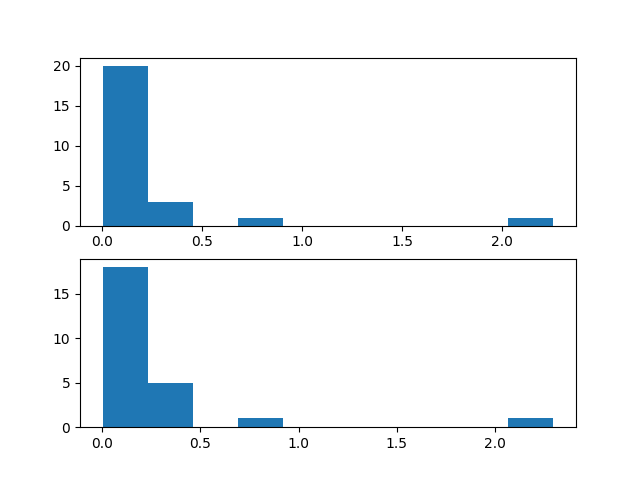
\includegraphics{forward_vs_adaptive.png}

    
\end{homeworkProblem}
\pagebreak
%Part 6%
\begin{homeworkProblem}
    \textbf{\large Statistical Significance}\\\\
    We will describe here a statistical hypothesis test for Part 5, so a method to determine whether the difference in performance between repeated forward A* and adaptive A* is significant. We claim that adaptive A* is on average faster than repeated forward A*. We start with a null hypothesis test: There is no difference in performance between repeated forward A* and adaptive A*. The goal is to determine whether the p values returned to us fall below an $\alpha = 0.05$ threshold, in which case we must reject the null hypothesis and conclude that there is indeed a difference in performance between the two algorithms. However, it is not enough to know that there is a significant difference, we also must determine the directionality of this difference- whether repeated forward A* is faster or adaptive A* is faster.
    \newline \newline
    To determine this significant, we use the t-test. First, we run repeated forward A* and adaptive A* on 50 grids, just as above. Next, we obtain their means and standard deviations. Next, we compute the t value using:
    \[t = \dfrac{\mu_1 - \mu_2}{\sigma_{comb}}\]
    where $mu_1$ is the mean of forward A*, $mu_2$ is the mean of adaptive A*, and $sigma_{comb}$ is the combined standard deviation, given by
    \[\sqrt{\dfrac{(N_1-1)(\sigma_1)^2 + (N_2-1)(\sigma_2)^2}{N_1 + N_2-2} \cdot (\dfrac{1}{N_1} + \dfrac{1}{N_2})} \]
    where $N_1$ and $N_2$ are given by the number of trials for repeated forward A* and adaptive A*, respectively (both are 50 in our case), and $\sigma_1$ and $\sigma_2$ are given by the standard deviations of forward and adaptive A*, respectively. Next, we perform a one sided t test (making sure to subtract the smaller mean from the greater mean) to determine the probability of the difference being significant in favor of the larger mean indeed being consistently larger. Note that we use the t test here and not the z test because we do not know the population standard deviation or mean, so we can't look at this data in terms of a general normal distribution for this type of experiment, and compare the difference in algorithm performance to the p value given by a z test.
    \newline\newline
    If we wanted to be particularly thorough, we could perform this trial multiple times and recover multiple p values, which we then apply Benjamini Hochberg/FDR correction to in order to account for multiple hypothesis testing, to obtain a p value that has undergone multiple rounds of simulating differences.
\end{homeworkProblem}

\end{document}